\chapter{Consideraciones sobre la implementación}

\section{Visión general}

En capítulo se hace referencia a las consideraciones sobre la implementación del proyecto, es decir, a los aspectos más significativos a la hora de codificar el sistema y sus funcionalidades. Se explicarán algunos de los pasos que se han dado a la hora de programar el sistema entero para que así, en caso de ser necesaria una expansión o revisión del proyecto, requiera emplear el menor esfuerzo posible a la hora de comprender lo que está desarrollado.

\section{Entorno de desarrollo}

Las herramientas que se han utilizado para facilitar la estructuración y desarrollo del proyecto han sido las siguientes:

\subsection{Git}

Git\cite{Git} es un software de control de versiones gratuito de código abierto diseñado por Linus Torvalds pensando en la eficiencia y la confiabilidad del mantenimiento de versiones de aplicaciones, más aún cuando estas tienen un gran número de archivos de código fuente, tanto de pequeños proyectos particulares como proyectos de grandes organizaciones. 

\begin{figure}[!htp]
	 \centering
	 
\includegraphics[scale=0.8]{fig/git_logo}
	 \caption{Logotipo de Git}
\end{figure}

Al principio, Git se pensó como un motor de bajo nivel sobre el cual otros pudieran escribir interfaces de usuario. Sin embargo, Git se ha convertido desde entonces en un sistema de control de versiones con funcionalidad plena. Hay algunos proyectos de mucha relevancia que ya usan Git, en particular, el grupo de programación del núcleo Linux.

Por otra parte la curva de aprendizaje de este sistema es relativamente baja, contando con una excelente documentación, pero más importante aún, al ser usado por muchos desarrolladores ha generado una comunidad de usuarios dispuesta a resolver cualquier problema.

En lo que respecta a este proyecto, se ha decidido usar los repositorios gratuitos ofrecidos por GitHub\cite{Github} para mantener el control de versiones de todo el código. El hecho de disponer una cuenta de estudiantes ha permitido hacer privados los repositorios para el almacenamiento seguro en la nube de forma gratuita.

\subsection{Sublime Text 2}

Sublime Text\cite{SublimeText} es un editor de texto y código fuente, escrito en C++ y Python, multiplataforma con una clara e intuitiva interfaz desarrollado especialmente para programadores que presenta varias características para mejorar la eficiencia de los desarrolladores. Entre estas ventajas cabe destacar el auto-completado, la capacidad de resaltar las expresiones propias de numerosos lenguajes, tales como \acrlong{js}, Python, \acrshort{html}, \acrshort{css}, visualizar más de un fichero a la vez por pantalla, etc. 

\begin{figure}[!htp]
	 \centering
	 
\includegraphics[scale=0.2]{fig/sublime_text_logo}
	 \caption{Logotipo de Sublime Text}
\end{figure}

Además, Sublime Text incluye una \acrshort{api} que permite desarrollar extensiones para dar soporte a más lenguajes o añadir nuevas herramientas y funcionalidades que hagan más sencilla la tarea de programar las aplicaciones.

\subsection{Google Chrome}

Google Chrome\cite{Chrome} es un navegador web desarrollado por Google\cite{Google} que incorpora herramientas para facilitar el desarrollo web para las distintas plataformas de sobremesa, tabletas y móviles.

\begin{figure}[!htp]
	 \centering
	 
\includegraphics[scale=0.4]{fig/chrome}
	 \caption{Logotipo de Google Chrome}
\end{figure}

Entre las características para el desarrollo web que dispone se ha utilizado el modo dispositivo y emulación móvil\cite{DeviceMode} que ha facilitado realizar las siguientes tareas:

\begin{itemize}
	\item Comprobar el diseño responsivo de la aplicación web en distintos tamaños de pantallas y resoluciones.
	\item Visualizar e inspeccionar el \acrshort{css} y las \textit{media queries}.
	\item Simular los eventos de entrada del dispositivo como las pulsaciones y la orientación de la pantalla.
\end{itemize}

En la siguiente figura (\ref{fig:google_device}) puede verse un ejemplo de la vista del entorno de desarrollo en Google Chrome.

\begin{figure}[!htp]
	 \centering
	 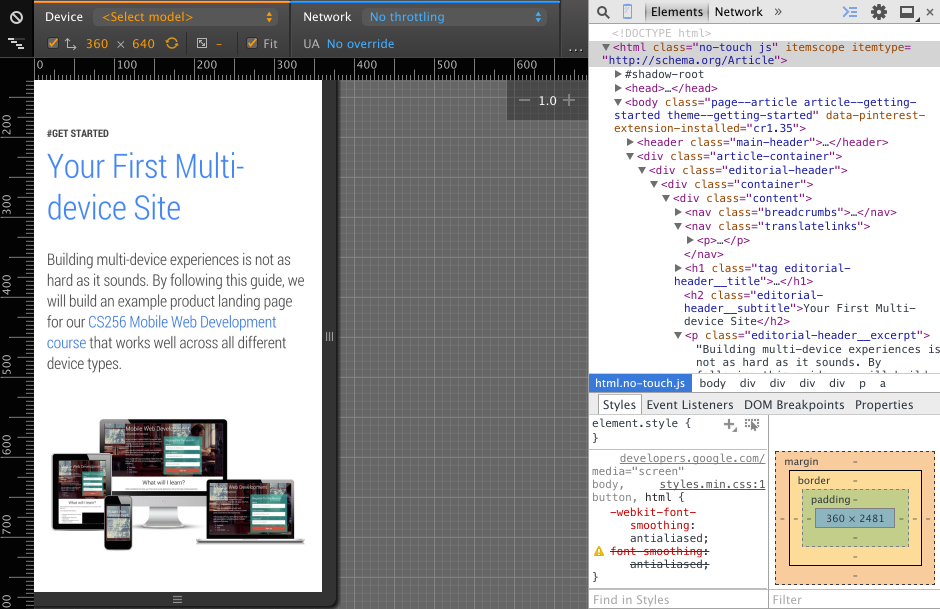
\includegraphics[scale=0.44]{fig/device_mode}
	 \caption{Modo dispositivo de Google Chrome}
	 \label{fig:google_device}
\end{figure}

\section{Calculo de la fecha de modificación para OAI-PMH}

El protocolo \acrshort{oaipmh} necesita de la fecha de creación o modificación de un recurso. Un cliente puede realizar una consulta a un servidor para que devuelva los recursos de rango temporal especificado, para poder obtener así lo últimos recursos que se han podido añadir al repositorio. Sin embargo, además de devolver los últimos recursos añadidos, el servidor retornará también todos los recursos que hayan sido modificado dentro del rango especificado.

Sin embargo el repositorio de \acrshort{labman} no ha sido diseñada con la capacidad de obtener la fecha de creación o de modificación de los recursos. Como primera solución ha este problema se decidió generar la fecha de creación del recurso en base a la fecha de publicación o de registro de la publicación y tesis doctoral. Como no había forma de comprobar la fecha de modificación, dado que la \acrshort{bd} contempla esta característica, se decidió hacer uso de los registros que almacena Django el su \textit{log} de administración dentro del repositorio de \acrshort{labman} con las tablas que pueden contemplarse en la figura \ref{fig:logsmodel}.

Como se puede ver en las tablas relacionadas con \textit{logs}, Django guarda el registro de cambios haciendo referencia a el identificador del registro, sin embargo como este puede no ser único entre las distintas tablas del modelo, se guarda también el nombre de ésta. Por lo que para calcular la fecha de modificación de una publicación, se requiere obtener todos los identificadores de las tablas a las que esté relacionado al igual que el nombre de las mismas. Una vez adquirida esta información se realiza una consulta a la tabla \textit{ContentType} para obtener el identificador que Django otorga a cada tabla y buscar en la tabla \textit{LogEntry} en busca de registros que coincidan con estos dos campos. Sí se encuentra se registra la fecha del registro (\textit{action\_time}) y se selecciona aquella con la fecha más alta de entre todo el conjunto de fechas de las tablas relacionadas con la publicación.

Dado que las tesis doctorales y las publicaciones están relacionadas con distintas tablas, se ha requerido definir dos métodos de consulta al \textit{log} de Django. En el algoritmo \ref{lst:busqueda_log_publicaciones} se muestra el proceso de búsqueda para las publicaciones

\begin{figure}[!htbp]
	\centering
	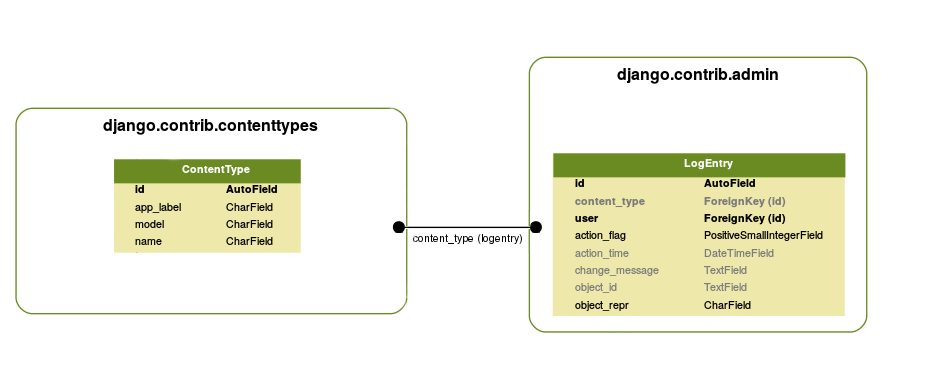
\includegraphics[scale=0.45]{fig/dbmodel/django_log}
	\caption{Modelo de datos relacional del sistema de ``logs'' de Django}
	\label{fig:logsmodel}
\end{figure}

\lstinputlisting[language=Python, frame=single, label={lst:busqueda_log_publicaciones}, caption= Búsqueda de la fecha de modificación más reciente para una publicación]{content/code/python/publication_log_search.py}

Debido a la volatilidad de los \textit{logs} y inneficiencia de buscar en los mismos por cada recurso se ha diseñado para su futura implementación una extensión del modelo de datos donde mediante \textit{triggers} se almacenen las fechas de modificación de los recursos  y así solo tener que hacer una \textit{Select} de la tabla donde se almacene el resultado de la fecha más reciente de las publicaciones.
Dicha implementación se propone el las lineas futuras de este documento, en la sección \ref{sec:future_lines}